\chapter{Materials and Methods}
\label{ch:methods}

  %% \epigraph{As palavras que nunca te direi.}{Translation of ``Message in a bottle''}
  %% \epigraph{The devil is in the details.}

  \section{Source of chemicals, enzymes, and solutions}
  All chemicals used were purchased from Sigma unless otherwise stated. All
  solutions were prepared according to \tref{tab:methods:solutions} with Milli-Q
  purified water, and autoclaved prior to use when appropriate.

  \begin{table}
    \captionIntro{Commonly used buffers and media}{}
    \label{tab:methods:solutions}
    \begin{description}
    \item[DMEM] \hfill \\
      \SI{4.5}{\g\per\l}   glucose;
      \SI{110}{\mg\per\l}  L-glutamine;
      \SI{584}{\ug\per\l}  sodium pyruvate;
      \SI{15.9}{\mg\per\l} phenol red.

    \item[DNA loading buffer (\SI{10}{\X})] \hfill \\
      \pcent{25} Ficoll ($w/v$);
      \SI{100}{\mM}      Tris--HCl pH=\num{7.4};
      \SI{100}{\mM}      EDTA.

    \item[FACS buffer] \hfill \\
      \pcent{96} DPBS ($v/v$); % 480.5 mL
      \SI{2}{\mM} EDTA;                         % 2 mL
      \SI{25}{\mM} HEPES buffer pH=\num{7.0};   % 12.5 mL
      \pcent{1} Fetal Calf Serum (FCS) ($v/v$).                    % 5 mL

    \item[Freezing media] \hfill \\
      \pcent{90} FCS ($v/v$);
      \pcent{10} DMSO ($v/v$).

    \item[Growth medium (HeLa, HEp2)] \hfill \\
      \pcent{89}            DMEM ($v/v$);   % 500ml
      \pcent{9}             FCS ($v/v$);    % 50ml
      \SI{1}{\X}            NEAA solution;  % 5.5mL
      \SI{50}{units\per\ml} penicillin;     % 5.5mL (Pen/Strep solution)
      \SI{50}{\ug\per\ml}   streptomycin.   % 5.5mL (Pen/Strep solution)

    \item[Growth medium (horse)] \hfill \\
      \pcent{81}            DMEM ($v/v$);   % 500ml
      \pcent{16}            FCS ($v/v$);    % 100ml
      \SI{2}{\X}            NEAA solution;  %  12mL
      \SI{50}{units\per\ml} penicillin;     % 5.5mL (Pen/Strep solution)
      \SI{50}{\ug\per\ml}   streptomycin.   % 5.5mL (Pen/Strep solution)

    \item[LB agar] \hfill \\
      \SI{20}{\g\per\l}  LB broth powder;
      \SI{7.5}{\g\per\l} agar.

    \item[LB broth] \hfill \\
      \SI{20}{\g\per\l} LB broth powder.

    \item[Running buffer] \hfill \\
      \SI{1}{\X}  TG;
      \pcent{0.1} SDS ($w/v$).

    \item[TAE (Tris Acetate EDTA)] \hfill \\
      \SI{40}{\mM} Tris;
      \SI{20}{\mM} acetic acid;
      \SI{1}{\mM}  EDTA.

    \item[TBS (Tris Buffered Saline)] \hfill \\
      \SI{50}{\mM} Tris--HCl pH=\num{7.5};
      \SI{100}{\mM}    NaCl.

    \item[TBS-T (TBS-Tween)] \hfill \\
      \pcent{99.95} TBS ($v/v$);
      \pcent{0.05}  Tween 20 ($v/v$).

    \item[TG (Tris Glycine)] \hfill \\
      \SI{25}{\mM}  Tris;
      \SI{192}{\mM} glycine.

    \item[Transfer buffer] \hfill \\
      \SI{1}{\X} TG;
      \pcent{15} methanol ($v/v$).
    \end{description}
  \end{table}

  Restriction enzymes, T4 DNA ligase, T4 Polynucleotide Kinase (PNK), and DNA
  ladders were obtained from New England BioLabs.
  Protein ladders were obtained from Invitrogen.

  For use in tissue culture, Fetal Calf Serum (FCS), and
  Dulbecco's Modified Eagle's Medium (DMEM) without phenol red and L-glutamine,
  were obtained from Lonza.  Non-Essential Amino Acid (NEAA) solution,
  Dulbecco's Phosphate-Buffered Saline (DPBS) without Ca$^{2+}$ and Mg$^{2+}$,
  and DMEM supplemented with glucose, sodium pyruvate, L-glutamine,
  and phenol red, were obtained from Sigma.
  Trypsin--EDTA and Penicillin--Streptomycin
  solution were obtained from Gibco.

  \section{DNA methods}
    \subsection{Bacterial cultures}
      \species{E.~coli} cultures were prepared with either LB broth or agar
      at \dc{37}. For antibiotic selection, ampicillin, kanamycin, and
      chloramphenicol, were used at concentrations of 100, 30,
      and \SI{34}{\mg\per\l} respectively.

    \subsection{Preparation of competent bacteria}
      Competent \species{E.~coli} cells were prepared from a culture of
      Invitrogen's One Shot TOP10 Chemically Competent \species{E.~coli}. LB
      cultures of \SI{1}{\l} were grown at \dc{37} until an OD$_{\SI{600}{\nm}}$
      of \numrange{0.4}{0.5}.  Subsequent steps were carried at \dc{4} with
      previously chilled equipment and solutions.

      Cultures were centrifuged at \SI{6000}{\gn} for 10 minutes, the
      pellet was resuspended in \SI{500}{\ml} of \SI{0.1}{\mM} CaCl$_2$, and
      incubated on ice for 30 minutes. The suspensions were centrifuged
      again at \SI{6000}{\gn} for 10 minutes,
      and the resulting pellet resuspended in
      \SI{100}{\ml} of CaCl$_2$ with \pcent{15} glycerol. Aliquots of
      competent cells were prepared and stored at \dc{-80}.

      Transformation efficiencies were measured after preparation of each
      batch and discarded if less than \SI{1d6}{\cfu\per\mg} of plasmid was
      obtained. Absence of antibiotic-resistant contaminations was assessed
      by streaking the cells on selective plates.

    \subsection{Transformation of competent cells}
      Competent cells were thawed on ice and split into aliquots of
      \SI{50}{\ul} to pre-chilled \SI{2}{\ml} tubes where
      \SI{1}{\ul} of \SI{\approx 100}{\ng\per\ul} DNA
      was added. Cells were incubated on ice for 30 minutes, followed by a
      60 seconds heat-shock at \dc{42}, and 5 more minutes on ice.
      \SI{300}{\ul} of non-selective LB was added to each tube and the
      cultures incubated at \dc{37} with vigorous shaking for 45 minutes.
      Samples from the cultures were then plated onto the appropriate
      antibiotic containing agar plates, and incubated overnight at \dc{37}.

      For concentrations of plasmid DNA higher than \SI{500}{\ng\per\ul}, only
      \SI{0.3}{\ul} of DNA was used, and both the initial and final incubation
      steps were shortened to 10 minutes.

    \subsection{Plasmid DNA preparation}
      Plasmid DNA was prepared with QIAprep Spin Miniprep,
      QIAGEN Plasmid \textit{Plus} Midi, QIAquick Gel Extraction, and QIAquick
      PCR purification kits from QIAGEN
      according the manufacturer's instructions.
      Once prepared, DNA was stored at \dc{-20}.
      DNA concentrations were measured
      with a NanoDrop 2000c spectrophotometer from
      Thermo Scientific.

    \subsection{Phenol:chloroform extraction}
      \label{sec:phenol-extraction}
      To purify DNA from whole cell extract,
      an equal volume of phenol:chloroform was
      added and the mixture centrifuged at \SI{6000}{\gn} for 15 minutes.
      The top aqueous phase was pipetted to a new tube and
      the process repeated a total of 3 times.

    \subsection{Ethanol precipitation}
      \label{sec:ethanol-precipitation}
      The DNA solution was mixed with \num{2.5} volumes of \pcent{100} ethanol
      and \num{1/10} volumes of Sodium Acetate (\SI{3}{\Molar}, pH=\num{5.2}),
      and incubated at \dc{4} for 15 minutes. When DNA concentrations were below
      \SI{50}{\ng\per\ul}, incubation was performed overnight.
      The DNA solution was then centrifuged at
      \SI{18000}{\gn} for 30 minutes at \dc{4} and the supernatant discarded.
      The pellet was left to dry until all traces of solvent evaporated.
      The DNA pellet
      was resuspended in the desired solvent:
      H$_2$O when being used for transfection,
      EB~buffer from QIAGEN in all other cases.

    \subsection{Agarose gel electrophoresis}
      Agarose gels with concentrations ranging from \SIrange{0.6}{2.0}{\percent}
      were prepared with TAE buffer, and supplemented with ethidium
      bromide to a concentration of \SI{200}{\ug\per\l}.
      DNA samples were loaded into the gel with DNA loading buffer and a
      choice of loading dyes between bromophenol blue, cresol red, orange G, or
      xylene cyanol.  In each case, the appropriate dye was chosen
      to avoid shadowing of the DNA bands. Electrophoresis was
      performed in Owl EasyCast electrophoresis chambers with
      \SI{1}{\X}~TAE buffer at
      \SIrange{80}{120}{\volt} until the required separation was achieved.
      Gels were visualised using a
      Alpha Innotech ChemiImager 5500 UV transilluminator.

    \subsection{DNA sequencing and oligonucleotide preparation}
      DNA sequencing was performed by LGC Genomics after cloning for sequence
      confirmation and avoiding unexpected mutations.

      Oligonucleotides were ordered from Eurofins MWG operon in lyophilised
      format, dissolved in H$_2$O to a \SI{100}{\micro\Molar} concentration,
      and stored at \dc{-20}. A list of all designed oligonucleotides is
      shown in \Aref{app:primers}.

    \subsection{Polymerase Chain Reaction}
      Different types of PCR experiments were performed for different purposes
      using a selection of DNA polymerases (\tref{tab:pcr-settings}).
      Taq polymerase with ThermoPol
      buffer was obtained from New England Biolabs.
      KOD Hot Start DNA polymerase with Mg$^{2+}$
      free buffer was obtained from Novagen. PCRs were performed on a
      Mastercycler epgradient thermocycler from Eppendorf.

      Use of different DNA polymerases was based on their cost-benefit for
      each application. For example, screening clones requires a large number
      of reactions in tandem and the introduction of small mutations
      is of no consequence. For these two reasons, the much cheaper Taq DNA
      polymerase was used for screening despite its relatively low fidelity and
      amplification rates. However, in PCR mutagenesis the whole plasmid
      is synthesised anew and we have no reasonable method to verify
      the entire plasmid
      sequence. As a result, KOD DNA polymerase was used for PCR mutagenesis.

      \begin{sidewaystable}
        \centering
        \captionIntro{PCR mixtures and conditions used}
          {
            Since each reaction was unique, with different pair of primers
            and template DNA, the optimal salt concentrations, temperature
            of the annealing step, and time of extension step actually used were
            sometimes different. Listed values correspond to the most common
            usage.
          }
        \label{tab:pcr-settings}

        \newcolumntype{W}{r<{\si{\second}}}
        \newcolumntype{T}{l<{\si{\degreeCelsius}}}

        \begin{tabular}{l W@{ at }T W@{ at }T W@{ at }T W@{ at }T W@{ at }T}
          \toprule
          \null                        & \multicolumn{4}{c}{cloning} & \crows{colony} & \crows{mutagenesis} & \crows{screening} \\
                                                \cmidrule(r){2-5}
          \null                        & \crows{genomic} & \crows{plasmid} \\
          \midrule
          Template (\si{\ng})          & \crows{1000}      & \crows{50}        & \crows{n/a}       & \crows{750}       & \crows{50}        \\
          DMSO (\si{\ul})              & \crows{---}       & \crows{---}       & \crows{1}         & \crows{---}       & \crows{1}         \\
          Buffer (\si{\X})             & \crows{1}         & \crows{1}         & \crows{1}         & \crows{1}         & \crows{1}         \\
          MgSO$_4$ (\si{\nmol})        & \crows{1.5}       & \crows{1.5}       & \crows{---}       & \crows{1.5}       & \crows{---}       \\
          dNTPs (\si{\mM} each)        & \crows{0.2}       & \crows{0.2}       & \crows{0.2}       & \crows{0.2}       & \crows{0.2}       \\
          Primer (forward) (\si{\uM})  & \crows{2}         & \crows{2}         & \crows{2}         & \crows{0.4}       & \crows{2}         \\
          Primer (reverse) (\si{\uM})  & \crows{2}         & \crows{2}         & \crows{2}         & \crows{0.4}       & \crows{2}         \\
          DNA polymerase (\si{U})      & \crows{0.5 (KOD)} & \crows{0.5 (KOD)} & \crows{2.5 (Taq)} & \crows{0.5 (KOD)} & \crows{2.5 (Taq)} \\
          \addlinespace
          Total volume (\si{\ul})      & \crows{25}        & \crows{25}        & \crows{25}        & \crows{25}        & \crows{25}        \\
          \addlinespace
          \midrule
          \addlinespace
          Initialization                & 120 & 94    & 120 & 94    & 180 & 94    & 120 & 94    & 120 & 94 \\
          Denaturation                  &  30 & 94    &  30 & 94    &  15 & 94    &  30 & 94    &  15 & 94 \\
          Annealing                     &  20 & 58    &  20 & 58    &  15 & 58    &  20 & 58    &  15 & 62 \\
          Extension (per \si{\kilo\bp}) &  30 & 68    &  20 & 72    &  60 & 72    &  30 & 68    &  60 & 72 \\
          Final extension               & 300 & 62    & 300 & 72    & 300 & 72    & 300 & 68    & 300 & 72 \\
          Final hold       & \crows{\dc{4}}      & \crows{\dc{4}}      & \crows{\dc{4}}      & \crows{\dc{4}}      & \crows{\dc{4}} \\
          Number of cycles & \crows{\SI{30}{\X}} & \crows{\SI{30}{\X}} & \crows{\SI{30}{\X}} & \crows{\SI{15}{\X}} & \crows{\SI{20}{\X}} \\
          \bottomrule
        \end{tabular}
      \end{sidewaystable}

      \subsubsection{Colony PCR}
        When screening multiple clones after transformation and a set of
        appropriate primers was available, PCRs were carried out directly on
        the bacteria colonies by adding them directly to the reaction mixture
        (\tref{tab:pcr-settings}). Bacteria from individual colonies were
        used to simultaneously perform a PCR and start a small culture.
        Plasmid purification was performed on cultures whose sample was
        confirmed to be the desired product by a positive PCR result.

      \subsubsection{Gene cloning}
        PCRs were used to clone and subclone genes from genomic DNA and
        plasmids, into different vectors. Primers were usually
        extended to introduce restriction sites and create DNA linkers.
        Additional extensions of cytosine and guanine were added to the
        5' end of primers to account for the minimum
        required \si{\bp} around the restriction sites as recommended
        by the restriction enzyme manufacturer, New England BioLabs.

      \subsubsection{Site-directed mutagenesis}
        Site-directed mutagenesis by PCR was used to insert or correct
        mutations in plasmids.
        Oligonucleotides were designed by flanking the
        desired mutation with regions at least \SI{16}{\bp} long
        and equal predicted melting temperature ($T_m$) of at least \dc{55}.
        When possible, the selected codon for mutation was the one
        with highest frequency in the organism used for expression
        in accordance with the
        codon usage database \citep{codon_usage}.
        To remove the template DNA post amplification, \SI{1.5}{\ul} of the
        restriction enzyme DpnI was added directly to the PCR mixture
        and incubated overnight at \dc{37}.
        Because DpnI requires the site to be methylated, it
        cleaves the template DNA which was synthesised in
        bacteria and leaves the newly \textit{in vitro}
        synthesised DNA.
        \SI{1}{\ul} of the digestion product was used for
        transformation directly without any clean up step.
        Individual clones were screened by sequencing.
        In PCR site-directed mutagenesis, the newly synthesised
        strands will be linear and so cannot be used as template for
        the following PCR cycle.
        This means that the amplification is linear rather than
        exponential and so the PCR is not actually a chain reaction.

      \subsubsection{Screening plasmid}
        PCRs were frequently used to screen plasmids for DNA sequences
        in the absence of opportune restriction sites or even plasmid maps.

    \subsection{Plasmid construction}
      \label{sec:plasmid-construction}

      \paragraph{pBOS--H2B--EGFP D25G V118I}
      Plasmid was provided by Prof.\@ Kevin Sullivan (NUIG) from
      previous work \citep{KevinH2BGFP}.  DNA sequencing identified
      gene \gene{HIST1H2BJ} as the closest human H2B in RefSeq but
      with missense mutations D25G and V118I.

      \paragraph{pBOS--H2B--EGFP}
      The D25G and V118I mutations in pBOS--H2B--EGFP were corrected
      by PCR mutagenesis using primers AFG114 and AFG115, and AFG112
      and AFG113 respectively.  The resulting product encodes the
      \gene{HIST1H2BJ} RefSeq gene.

      \paragraph{pBOS--EGFP}
      The pBOS--H2B--EGFP was digested with KpnI and BamHI and the
      band corresponding to the linearised vector, without the H2B
      sequence, was purified by gel extraction.  This linearised vector
      was used as backbone vector for the other pBOS constructed
      plasmids.

      \paragraph{pBOS--H2A--EGFP}
      The \gene{HIST1H2AB} gene sequence was amplified from HeLa
      genomic DNA with primers AFG116 and AFG118, the PCR product
      digested with KpnI and BamHI, and then ligated into the
      pBOS--EGFP vector.  The \gene{HIST1H2AB} was chosen because it
      encodes the same protein as the H2A used in previous work
      \citep{flaus2004sin}.  The only other available alternative
      that encoded the same protein was \gene{HIST1H2AE}.
      However, the \gene{HIST1H2AE} sequence has a lower codon
      adaptation index and more stable predicted 5' mRNA secondary structure.
      An accidental frameshift mutation near the stop codon was
      posteriorly fixed by PCR mutagenesis using primers AFG396 and
      AFG397.

      \paragraph{pBOS--H2AX--EGFP}
      The \gene{H2AFX} gene sequence was amplified from HeLa genomic
      DNA with primers AFG130 and AFG131.  The same strategy used in
      the cloning of pBOS--H2A--EGFP was used.  An accidental
      frameshift mutation near the stop codon was posteriorly fixed by
      PCR mutagenesis using primers AFG400 and AFG401.

      \paragraph{pBOS--H2AX--EGFP S139 mutants}
      For H2AX S139 mutations, the \gene{H2AFX} gene sequence was
      amplified from HeLa genomic DNA in the same reaction that the
      mutations were introduced since their location is close to the
      sequence 3' end.  Primers AFG132, AFG133, and AFG134, were used
      with AFG130 to introduce H2AX mutations S139A, S139D, and S139E
      respectively.  The mutation to alanine blocks phosphorylation of
      S139, while mutation to aspartic and glutamic acid mimic
      phosphorylation of S139.  The same strategy used in the cloning
      of pBOS--H2AX--EGFP was used, including the correction of a
      frameshift mutation with AFG400 and AFG401.

      %% Note: not gene sequence so we don't talk about the gene and
      %%       therefore not in italic (and we don't use \gene)
      \paragraph{pBOS--H2A.Z--EGFP}
      Due to the presence of introns in the \gene{H2AFZ} gene
      sequence, the transcript sequence was amplified from HeLa cDNA
      provided by Dr.\@ Nadine Quinn \citep{NadineThesis}.  The
      amplification was performed with primers AFG121 and AFG122, and
      the product cloned into the pBOS--EGFP with the same strategy
      used for pBOS--H2A--EGFP.
      An accidental frameshift mutation near the stop codon was
      posteriorly fixed by PCR mutagenesis using primers AFG398 and
      AFG399.

      \paragraph{pBOS--H3--EYFP.MC--N1}
      Plasmid was provided by Prof.\@ Kevin Sullivan (NUIG).  DNA
      sequencing identified the H3 sequence as the human RefSeq
      \gene{HIST1H3B} gene, encoding H3.1 from histone cluster 1.

      \paragraph{pBOS--H3--EYFP T45A and T45E}
      Mutations to H3 T45 were inserted into pBOS--H3--EYFP.MC--N1 by
      PCR mutagenesis. The primers AFG151 and AFG152 were used
      to generate the
      T45E mutation, and AFG153 and AFG154 for T45A.

      \paragraph{pBOS--H4--ECFP.M--N1}
      Plasmid was provided by Prof.\@ Kevin Sullivan (NUIG).  DNA
      sequencing identified the H4 sequence as the human RefSeq
      \gene{HIST1H4J} or \gene{HIST1H4K}, both of which have the same
      genomic sequence.

      \paragraph{pBOS--H4--ECFP R45H}
      The H4 R45H mutation was inserted into pBOS--H4--ECFP.M--N1 by
      PCR mutagenesis using the primers AFG124 and AFG125. The codon
      \texttt{CAC} was selected for the histidine amino acid due to
      its higher codon usage in the human genome \citep{codon_usage}.

      \paragraph{pBOS--H4--EYFP}
      The plasmid pBOS--H3--EYFP.MC--N1 was digested with the
      restriction enzymes BamHI and NotI to extract the EYFP sequence
      which was purified by agarose gel extraction.  The pBOS--H4
      sequence was prepared in the same manner from
      pBOS--H4--ECFP.M--N1.  The two fragments were ligated to
      construct pBOS-H4-EYFP.

      \paragraph{pBOS--H4--EYFP R45H}
      The same strategy used for the cloning of wild type
      pBOS--H4--EYFP was used for the R45H mutant using
      pBOS--H4--ECFP R45H.

      \paragraph{PA-GFP}
      The PA-GFP sequence used as an insert for other plamids was
      amplified from pPA-GFP--N1 with primers AFG478 and AFG479.  The
      amplicon was purified by agarose gel extraction, digested with
      NotI and BamHI, and then cleaned by PCR purification.  The
      pPA-GFP--N1 plasmid was a kind gift from Chelly van Vuuren
      (NUIG).

      \paragraph{pBOS--H2B--PA-GFP}
      The plasmid pBOS--H2B--EGFP was digested with NotI and BamHI
      which removed the EGFP sequence.  The vector was purified by
      agarose gel extraction and ligated with the PA-GFP insert.  This
      strategy introduced a proline to arginine mutation in the linker
      sequence between H2B and PAGFP when compared to the linker
      sequence between H2B and EGFP.
      %% This mutation in the H2B linker (DPPVAT to DPRVAT) was not on
      %% purpose but wasn't an accident either.  We knew about it and
      %% could have easily avoid it but would cost us one extra primer
      %% and it shouldn't be making a difference.

      \paragraph{pBOS--H3--PA-GFP}
      The plasmid pBOS--H3--EYFP.MC--N1 was digested with NotI and
      BamHI which removed the EYFP sequence.  The vector was purified
      by agarose gel extraction and ligated with the PA-GFP insert.
      %% Unlike the H2B--PA-GFP plasmid, this did not introduce any
      %% mutation in the linker sequence.

      \paragraph{mCherry--\textalpha--tubulin}
      Plasmid was a kind gift from Chelly van Vuuren (NUIG).

      %% I'm actually not sure if Kevin gave me the pMH3.2--614 or the
      %% pCA-TAG plasmid. I did not have any plasmid map or sequence, only
      %% the very small Figure 5 of his paper PMID:9024683
      %% I couldn't even use any standard sequencing primer and by the time
      %% we cloned our genes there, we had already decided to kill the project
      %% so we never got to actually try these in human cells.
      \paragraph{pMH3.2--614}
      The plasmid includes a mouse replication dependent histone H3.2
      gene with upstream and downstream regulatory elements
      \citep{pMH3-plasmid}.  It was provided by Prof.\@ Kevin
      Sullivan.  Due to the absence of convenient restriction sites in
      the plasmid, insertion of alternative histone gene sequence was
      performed by blunt-end ligation of PCR products.  pMH3.2--614
      was amplified with primers AFG417 and AFG418 which amplified the
      vector backbone, including the upstream and downstream
      regulatory elements but ignored the H3.2 coding sequence.  The
      amplified sequence was purified by agarose gel extraction to be
      used in the cloning of pM-H2B--EGFP and pM-H3--EYFP.

      \paragraph{pM-H2B--EGFP and pMH3--EYFP}
      The H2B--EGFP insert sequence was generated by PCR amplification
      with primers AFG419 and AFG420, purified by agarose gel
      extraction, and ligated into the pMH3.2--614 vector.  The
      primers for the insert, AFG419 and AFG420, were phosphorylated
      by T4~PNK prior to PCR since T4~PNK is more efficient on single
      stranded DNA.
      The same strategy was used for the cloning of pMH3--EYFP using
      primers AFG424 and AFG420.

  \section{Protein methods}
    \subsection{Western blotting}
      \subsubsection{Protein concentration determination}
        Concentration of protein was measured with Bradford reagent.
        \SI{2}{\ul} of the sample after sonication (\Sref{sec:cell-extract})
        was mixed with \SI{48}{\ul} of H$_2$O and \SI{50}{\ul} of NaOH and
        incubated at \dc{65} for 8 minutes before adding \SI{900}{\ul} of
        Bradford reagent from Pierce. The mixture was transferred to plastic
        cuvettes and the absorbance at \SI{595}{\nm} measured in a Shimadzu
        spectrophotometer. The values obtained were interpolated from a
        standard curve prepared using known concentrations of BSA.

      \subsubsection{SDS--PAGE}
        Resolving and stacking SDS--PAGE gels of \SIrange{15}{5}{\percent}
        respectively, both with a cross-linking ratio of \num{37.5}:1 as
        described in \citet{harlow_electrophoresis_1988} were used. The
        resolving gel was poured directly after addition
        of TEMED and it was covered with a layer of isopropanol during polymerisation
        to ensure a sharp interface between the resolving and stacking layers.
        Protein samples and markers were boiled at \dc{99} for 3 minutes and each
        was loaded twice, with volumes for \SI{3.3}{\ug} and \SI{16.5}{\ug} of
        protein. Gels ran at \SI{180}{\volt} for 1 hour in \SI{1}{\X} TG buffer.

      \subsubsection{Protein transfer}
        Protein transfer occurred through the wet transfer system. The
        SDS-PAGE gel was placed onto pre-cut nitrocellulose transfer membrane
        previously soaked in transfer buffer. It was then set between a pair
        of extra thick blotting paper and cushions before being placed inside
        a transfer apparatus. The transfer ran at \dc{4} for 60
        minutes at \SI{100}{\volt}.

      \subsubsection{Probing of blot with antibody}
        Blocking of the membrane was performed with \SI{10}{\percent}
        non-fat dry milk (Marvel) in \SI{1}{\X} TBS-T buffer
        at room temperature for 30 minutes. Blocking was followed by
        primary antibody incubation which occurred in \SI{5}{\percent} non-fat
        dry milk in \SI{1}{\X} TBS-T overnight at \dc{4}. Concentrations of
        antibody used were 1:500 and 1:20000 for anti-GFP (catalogue
        number 11~814~460~001 from Roche) and anti-H3 (code ab1791 from
        abcam). The membrane was then washed with \SI{1}{\X} TBS-T for
        15 minutes 3 times before secondary antibody incubation
        in \SI{5}{\percent} non-fat dry milk with \SI{1}{\X} TBS-T for
        1 hour. The membrane was washed once more in the same
        conditions as before for the detection. All blocking, antibody
        incubation and washing steps occurred on a rocker.

        Detection was performed using the SuperSignal West Pico Chemiluminescent
        Substrate from Pierce, adding 1:1 of the solutions and allowing it to incubate
        with the membrane for 5 minutes. The membrane was exposed to x-ray films for
        10, 60, 5, 180 and 1800 seconds which were then developed.


  \section{Cell methods}
    \subsection{Cell culture}
      HeLa (ATCC CCL-2) and HEp-2 cells were supplied by
      Dr.\@ Agnieszka Kaczmarczyk \citep{AgaThesis}
      and Dr.\@ Volker Döring \citep{VolkerThesis} respectively.
      Primary horse fibrolasts were a gift from Prof.~Elena Giulotto from the
      University of Pavia, Department of Genetics and Microbiology.

      All cell lines were maintained at \dc{37}
      and \pcent{5} CO$_2$ in \SI{10}{\cm}
      diameter plates with \SI{10}{\ml} of their respective growth
      medium \trefp{tab:methods:solutions}.
      Once cells reached a confluence of \SIrange{80}{90}{\percent},
      they were trypsinised and split.  First they were washed with
      DPBS and then
      incubated at \dc{37} for 5 minutes in \SI{2}{\ml} of
      trypsin--EDTA.  Finally, they were diluted 1:10 in fresh media
      and transferred to a new plate.

    \subsection{Cell stock storage}
      For long-term storage of HeLa cell lines, they were grown until
      they reached a confluence of \SIrange{80}{90}{\percent} and then
      trypsinised. A volume of Freezing Media was added, equal
      to the volume of trypsin--EDTA, and \SI{2}{\ml} aliquots of
      cells transferred to cryotubes. Tubes were immediately wrapped in
      cotton and placed at \dc{-80}.

    \subsection{Whole cell extract}
      \label{sec:cell-extract}
      To obtain whole cell extracts, HeLa cells were trypsinised as usual. Growth
      medium added and the suspension was centrifuged at \SI{900}{\gn}
      for 10 minutes.
      Subsequent steps were carried out at \dc{4} and with previously
      chilled reagents. The supernatant was discarded and the pellet
      resuspended in \SI{500}{\ul} of chilled PBS before being
      sonicated 3 times at \pcent{40} amplitude for 10 seconds. Avoiding the
      formation of foam at the top, \SI{300}{\ul} of suspension was transferred
      from the bottom of the tube to a new \SI{1.5}{\ml} tube
      and mixed with an equal
      volume of Laemmli buffer before being stored at \dc{-80}.
      \SI{2}{\ul} from the suspension was also transferred to a new tube
      for determination of protein concentration by Bradforf protein assay.

    \subsection{Genomic DNA extraction}
      To extract genomic DNA from HeLa cells, they were trypsinised and
      growth medium was added before counting with an hemocytometer.
      Cells were centrifuged at \SI{1500}{\gn} for 10 minutes at \dc{4}, the
      supernatant was discarded
      and the pellet resuspended in TE buffer to achieve
      a desired concentration of \SI{4e7}{cells\per\ml}. 9 volumes of
      genomic lysis buffer was added
      and the mixture was incubated at \dc{37} for
      90 minutes. Proteinase K was then added to a final concentration of
      \SI{100}{\ug\per\ml} and the mixture was
      incubated at \dc{50} for 3 hours and
      swirled every 20 minutes. DNA was then purified by
      phenol:chloroform extraction \Srefp{sec:phenol-extraction} and ethanol
      precipitation (\Sref{sec:ethanol-precipitation}).

    \subsection{Viable cells count}
      Trypan blue was used to assess the number of viable cells.
      After trypsinisation, cells were diluted in growth media,
      to a final concentration of \SI{2e5}{cells\per\ml}.
      To \SI{0.5}{\ml} of the cell suspension, \SI{0.1}{\ml} of \pcent{0.4}
      Trypan Blue Stain was added and the mixture left for 5 minutes
      at room temperature before counting
      the cells in an hemocytometer and making a distinction between
      stained (non-viable) and non-stained (viable) cells.

    \subsection{Kill curve}
      \label{sec:methods:kill-curve}
      Cells were trypsinised and plated at \pcent{25} confluence on
      a 24-well plate. After 24 hours, medium was replaced using different
      concentrations of the antibiotic per well, 3 replicas for each.
      After 3 days, medium was replenished
      with the same antibiotic concentrations. After 4 days, a total of
      one week after addition of antibiotics, cells were trypsinised and a count
      of viable cells was performed with
      Trypan Blue.

      The highest concentration tested with no viable cells in all
      replicas after 7 days was used for selection of transfected
      cells when establishing stable cell lines.

    \subsection{Transfection by lipofection}
      \label{methods:lipofection}
      Cells were transfected using Lipofectamine~2000, a cationic lipid
      reagent, from Invitrogen. Cells were trypsinised as usual on the
      day before transfection and replated on 6 well plates (surface area
      of \SI{9.5}{\square\cm\per well}) with \SI{2.5}{\ml} of growth
      medium so they would be \SI{90}{\percent} confluent on the following
      day. For each well, two tubes with \SI{250}{\ul} of transfection
      medium were prepared, one with \SI{7.5}{\ul} of Lipofectamine~2000
      and another with \SI{3750}{\ng} of DNA from a stock with concentration
      of \SI{500}{\ng\per\ul} and prepared by ethanol precipitation
      (\Sref{sec:ethanol-precipitation}).
      Both tubes were incubated at room temperature for 5 minutes,
      mixed together, and incubated again at room temperature for 20 minutes. Cells
      were washed with DPBS during this time and growth medium switched to \SI{2}{\ml}
      of transfection medium. The mixture was then added to the cells medium who
      were incubated at \dc{37} for 6 hours after which time it was switched back to
      \SI{0.5}{\ml} of growth medium.

    \subsection{Transfection by electroporation}
      Cells were transfected by electroporation using an Amaxa nucleofector
      device with Ingenio Electroporation solution and cuvettes from Mirus Bio.
      Cells were grown to confluence and trypsinised as usual. Growth medium was
      added to a total volume of \SI{8}{\ml}, and \SI{1}{\ml} aliquots (for
      approximately \SI{10e6}{cells}) were centrifuged at \SI{160}{\gn} for 5~minutes.
      The supernatant was discarded and a volume of \SI{2}{\ul} of plasmid at
      a concentration of \SI{500}{\ng\per\ul} was added to the top of the pellet.
      The cell pellet was resuspended in \SI{100}{\ul} of Mirus Bio Ingenio
      Electroporation solution and transferred to \SI{0.2}{\cm} cuvettes for
      electroporation in an Amaxa nucleofector. According to the manufacturers
      instructions, the preset programs I-013 and O-17 were used to transfect
      HeLa and HEp-2 cells respectively.

    \subsection{Generation of stable cell lines}
      Cells were trypsinised and split to a low confluence (1:20) on
      \SI{10}{\cm} dishes 24~hours after transfection.  After another
      24 hours, the appropriate antibiotic was added to the medium
      with a final concentration as determined by performing an
      antibiotic kill-curve.  Cell
      growth was observed daily followed and medium replaced every 3
      days.  As cell colonies started to be visible by the naked eye,
      approximately 3~weeks after plating, these were screened by
      fluorescence microscopy.  Positive colonies were aspirated and
      moved into 24-well plates with \SI{1}{\ml} disposable pipette
      tips, and the thinnest extremity removed.  Mixed populations
      were observed, so the cells with highest expression levels were
      FACS sorted to obtain homogeneous populations
      \frefp{fig:methods:facs}.

    \subsection{Fixation and staining}
      For microscopy visualisation, HeLa cells were grown directly
      on HCl washed coverslips as they
      have difficulty attaching to glass. At least 24 hours post
      plating and fixation, growth medium was removed and the cells
      washed with PBS once before incubation with \SI{4}{\percent} formaldehyde in PBS
      for 4 minutes. This solution was then removed
      and the cells washed with H$_2$O two more
      times, after which coverslips were removed from the wells and left to air dry.
      For each coverslip, \SI{2}{\ul} of SlowFade Light Antifade kit from Molecular Probes
      was used for mounting the coverslip on a microscope slide. DAPI was added
      to the mounting media when needed. Coverslips were then sealed with a 1:1
      mixture of clear nail polish and acetone and stored on a dark box at \dc{4}.

    \subsection{Flow cytometry}

      Cells were trypsinised and after addition of medium, centrifuged
      at \SI{160}{\gn} for 5~minutes. The supernatant was discarded and the
      pellet washed with PBS. The sample was centrifuged one more time at
      \SI{160}{\gn} for 5~minutes. The supernatant was discarded again
      and the new
      pellet resuspended in Fluorescence-Activated Cell Sorting (FACS) buffer.

      Populations with mixed levels of fluorescent intensity were
      frequently obtained while preparing stable cell lines. In such
      cases, cells with similar intensity of their corresponding
      fluorophore were sorted by FACS \frefp{fig:methods:facs}.

      \begin{figure}
        \centering
        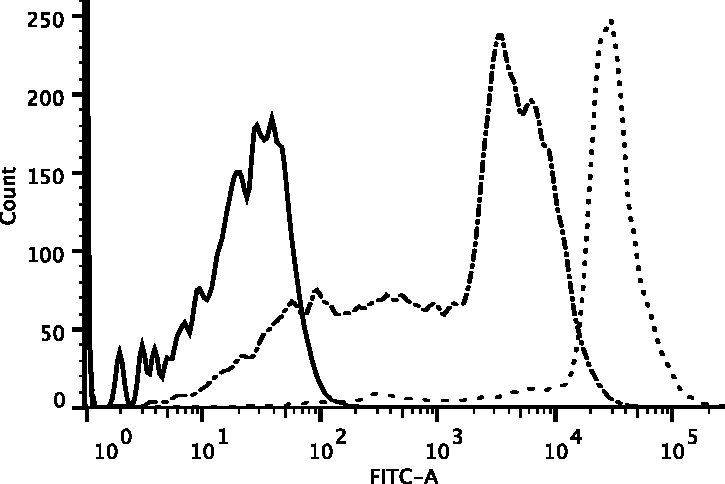
\includegraphics[width=\textwidth]{figs/facs-stable-cell-lines.pdf}
        \captionIntro{Fluorescent intensity of HeLa cell populations
          by flow citometry}%
                     { The multiple populations with differing
                       intensity values were sorted by FACS. The full
                       line represents the intensity profile of HeLa
                       wild type cells, the dash-dot line the mixed
                       population of HeLa cells expressing H2B--EGFP,
                       and the dotted line the homogeneous cell
                       population after sorting.  }
        \label{fig:methods:facs}
      \end{figure}

      Both sample analysis and cell sorting were performed with live cells, the
      first with a BD FACSCanto~II, and the later with a BD FACSAria~II.

  \section{Software used}
    \label{sec:methods:software}
    Image analysis was performed using GNU Octave version \OctaveVersion{},
    and Octave Forge Image, Optim, Statistics, Bioformats, and Signal
    packages, versions \OctaveImageVersion{}, \OctaveOptimVersion{},
    \OctaveStatisticsVersion{}, \OctaveBioformatsVersion{}, and
    \OctaveSignalVersion{} respectively.

    ImageJ, as distributed by the Fiji project, was routinely used
    for microscope image visualisation.  PyMOL, by Schrödinger, LLC,
    was used for visualisation of protein structures.
    The European Molecular Biology Open Software Suite (EMBOSS)
    was used for analysis of codon usage, RNA folding, and reading of
    chromatogram files.

  \section{Source Code and Data}
    Source code to reproduce this thesis is available online,
    including its entire development history as a git repository, at
    \url{https://github.com/carandraug/phd-thesis.git}.  The SCons build
    system is used to automate the build.  Multiple dependencies will
    be required, namely GNU Octave, the Octave Forge Image package,
    BioPerl, and the Perl Bio-EUtilities module distribution, all of
    which will be confirmed by SCons.  All the data required for the
    build is available online at Zenodo with record ID 377035 and
    DOI \texttt{10.5281/zenodo.377035}.  The script
    \command{bootstrap.sh} is included in the thesis repository and
    can be used to download all data into the correct locations.

  \section{Developed software}
    Multiple pieces of software were developed in the course of this
    thesis.  When appropriate, these were contributed and merged into
    the software used \Srefp{sec:methods:software}.  Such work is
    described in \Cref{ch:software}.
